% siminos/spatiotemp/chapter/zeta2D.tex
% $Author: predrag $ $Date: 2021-12-24 01:25:20 -0500 (Fri, 24 Dec 2021) $

\chapter{Zeta functions in 2D}
\label{chap:zeta2D}
% extracted from Ising.tex  2020-12-20

\renewcommand{\ssp}{\ensuremath{\phi}}             % lattice site field
\renewcommand{\Ssym}[1]{{\ensuremath{m_{#1}}}}    % Boris

``symbols'' are sometimes called ``colors''.             \toCB

    \PC{2016-10-11}{From {Ban} \etal\rf{BHLL11}, on two-dimensional
    $\mathbb{Z}^{2}$-shifts of finite type}
Let $\mathbb{Z}^{2}$ be a two-dimensional planar lattice. For any $m,n\geq 1$ and
$(i,j)\in\mathbb{Z}^{2}$, the $m\times n$ rectangular lattice with the
left-bottom vertex $(i,j)$ is denoted by
\[
\mathbb{Z}_{m\times n}((i,j))
=\left\{(i+m',j+n')\mid 0\leq m'\leq m-1,0\leq n'\leq n-1 \right\}
\,.
\]
and
\(
\mathbb{Z}_{m\times n}=\mathbb{Z}_{m\times n}((0,0)).
\)
Let $\mathcal{S}_{p}$ be an alphabet of $p$ ($\geq 2$) symbols. For $m,n\geq 1$,
$\Sigma_{m\times n}(p)=\mathcal{S}_{p}^{\mathbb{Z}_{m\times n}}$ is the set
of all $m\times n$ local patterns or rectangular blocks, and
$\Sigma_{m\times n}(\mathcal{B})$ is the set of admissible  $m\times n$  patterns.
$\Sigma(\mathcal{B})$ is the set of all admissible patterns in
$\mathcal{B}$.


\begin{description}
    \PCpost{2016-11-07} {
There is much literature on multi\dmn\
shifts\rf{Ward94,ChoMal95a,ChoMal95b,ChMaVanV96,ChMaSh98,
Friedland97,QuaTro00,BanLin05,BanLinLin07,BoyPavSch10,HocMey10,BHLL11,HuLin11,
BHLL13,HuLin16}.
It does not seem to directly relevant to the 2\dmn\
{\spt} symbolic dynamics studied by us.
    }


    \PCpost{2016-05-04}{
There is much literature on multi-dimensional shifts
that we have to understand (or at least understand whether it is relevant to
our 2\dmn\ symbolic dynamics):

Ward\rf{Ward93} {\em An algebraic obstruction to isomorphism of {Markov}
shifts with group alphabets} introduced $Z^2$-subshift, or
the space of doubly indexed sequences over a finite abelian compact group G.

Ward\rf{Ward94}
 {\em Automorphisms of {$\integers^d$}-subshifts of finite type}

Ward and Miles\rf{WarMil11}
{\em A directional uniformity of periodic point distribution and mixing}: ``
For mixing actions generated by commuting automorphisms of a compact
abelian group, we investigate the directional uniformity of the rate of
periodic point distribution and mixing. When each of these automorphisms
has finite entropy, it is shown that directional mixing and directional
convergence of the uniform measure supported on periodic points to Haar
measure occurs at a uniform rate independent of the direction.
''

Miles and Ward\rf{MilWar16} {\em The dynamical zeta function for
commuting automorphisms of zero-dimensional groups}: ``
For a $\integers^d$-action $\alpha$ by commuting homeomorphisms of a
compact metric space, Lind\rf{Lind96}, \CBlibrary{Lind96} introduced a
dynamical zeta function that generalizes the dynamical zeta function of a
single transformation. We investigate this function when $\alpha$ is
generated by continuous automorphisms of a compact abelian
zero-dimensional group. We address Lind's conjecture concerning the
existence of a natural boundary for the zeta function and prove this for
two significant classes of actions, including both zero entropy and
positive entropy examples. The finer structure of the periodic point
counting function is also examined and, in the zero entropy case, we show
how this may be severely restricted for subgroups of prime index in
$\integers^d$.
''

Ward and Miles\rf{WarMil15}
{\em Directional uniformities, periodic points, and entropy}: ``
For dynamical systems generated by $d\geq2$ commuting homeomorphisms,
dynamical invariants like entropy and periodic point data, become more
complex and permit multiple definitions. A powerful theory of directional
entropy and periodic points can be built. An underlying theme is
uniformity in dynamical invariants as the direction changes, and the
connection between this theory and problems in number theory; we explore
this for several invariants and highlight Fried's notion of average
entropy and its connection to uniformities in growth properties.
''




Al Refaei 2011
%http://dx.doi.org/1O.3923/ajms.2011 (?)
``The group $Z^2$ acts natural on the space ?? via left and upward shifts"
is gibberish, ignore it.

Roettger\rf{Roettger05},
{\em Periodic points classify a family of Markov shifts}, writes:

Ledrappier introduced the following type of space of doubly indexed
sequences over a finite abelian group G,
\[
X_G=\{(x_{s,t}) \in G^{\integers^2} | x_{s,t+1}=x_{s,t}+x_{s+1,t}
\quad \mbox{for all }s,t\in \integers\}.
\]
The group $\integers^2$ acts naturally on the space $X_G$ via left and upward shifts.

Chow, Mallet-Paret and Van Vleck\rf{ChoMal95a,ChoMal95b,ChMaVanV96,ChMaSh98}
{\em Pattern formation and spatial chaos in spatially discrete evolution equations}

(Actually, Bunimovich might have worked on this)

Friedland\rf{Friedland97}
{\em On the entropy of {$\integers^d$} subshifts of finite type}

Quas and Trow\rf{QuaTro00}
{\em Subshifts of multi-dimensional shifts of finite type}

Desai\rf{Desai06}
{\em Subsystem entropy for $\integers^d$ sofic shifts}

{Ban} and {Lin}\rf{BanLin05,BanLinLin07} {\em Patterns generation and transition
matrices in multi-dimensional lattice models}

Boyle, Pavlov and Schraudner\rf{BoyPavSch10}
{\em Multidimensional sofic shifts without separation and their factors}

Hochman and Meyerovitch\rf{HocMey10}
{\em A characterization of the entropies of multidimensional shifts of finite type}

{Ban}, {Hu}, {Lin}, and {Lin}\rf{BHLL11}, {\em Verification of mixing
properties in two-dimensional shifts of finite type}

Hu and Lin\rf{HuLin11}
   {\em Nonemptiness problems of plane square tiling with two colors}

Hu and Lin\rf{HuLin16},
 {\em On spatial entropy of multi-dimensional symbolic dynamical systems},
discuss multi-dimensional shift space for a rectangular spatial entropy
which is the limit of growth rate of admissible local patterns on finite
rectangular sublattices.
    }

    \PCpost{2016-05-04}{
{Ban}, {Hu}, {Lin}, and {Lin}\rf{BHLL13},
{\em Zeta functions for two-dimensional shifts of finite type}
seems to be a \HREF{http://bookstore.ams.org/memo-221-1037} {must read},
with exhaustive references. The zeta functions of two-dimensional shifts
of finite type which generalizes the Artin-Mazur\rf{ArtMaz65} zeta
function was given by Lind\rf{Lind96}, \CBlibrary{Lind96} for
$\integers^2$-action. The rotationally symmetric trace operator is the
transition matrix for x-periodic patterns with period $n$ and height 2.
The rotational symmetry induces the reduced trace operator, and the zeta
function in the $x$-direction is now a reciprocal of an infinite product
of polynomials. The zeta function can be presented in the $y$-direction
and in the coordinates of any unimodular transformation in
$GL_2(\integers)$. Therefore, there exists a family of zeta functions
that are meromorphic extensions of the same analytic function. The Taylor
series for these zeta functions at the origin are equal with integer
coefficients, yielding a family of identities, which are of interest in
number theory.

Their \textbf{Example 7.2}\\
Let $F_2 = \{0, 1\}$ and
\[
\mathbb{Z} =
\left\{
\ssp_{n\zeit}
    =
       \ssp_{n,\zeit+1} + \ssp_{n,\zeit-1}
     + \ssp_{n+1,\zeit} + \ssp_{n-1, \zeit}
\mbox{ for all } n\zeit\in\integers^2
\right\}
\] % \ee{CL18:CatLattT=1}
is about the harmonic patterns on square-cross lattice
$\lattice$ studied by\\
F. Ledrappier, \emph{Un champ markovien peut {\^{e}}tre d'entropie nulle et
m{\'e}langeant}, C. R. Acad. Sc. Paris Ser. A 287 (1978), 561-562.
For us, this is a bit strange - our `harmonic' value would be $4\ssp_{n\zeit}$,
not $\ssp_{n\zeit}$.
    }


%%%%%%%%%%%%%%%%%%%%%%%%%%%%%%%%%%%%%%%%%%%%%%%%%%%%%%
\begin{figure}[h]
    \begin{center}
\begin{minipage}[height=.20\textheight]{.18\textwidth}
\centering
\includegraphics[width=.75\textwidth]{cylinderTime1}
    \vfill
\small{\texttt{(a)}}
\end{minipage}
~~~~
\begin{minipage}[height=.20\textheight]{.75\textwidth}
\centering
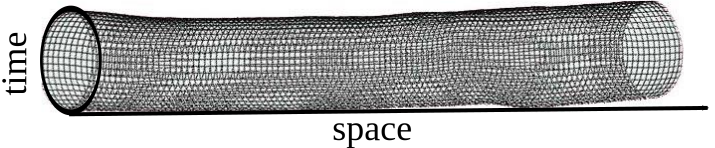
\includegraphics[width=.80\textwidth]{cylinderSpace1}
\\
\small{\texttt{(b)}}
\\
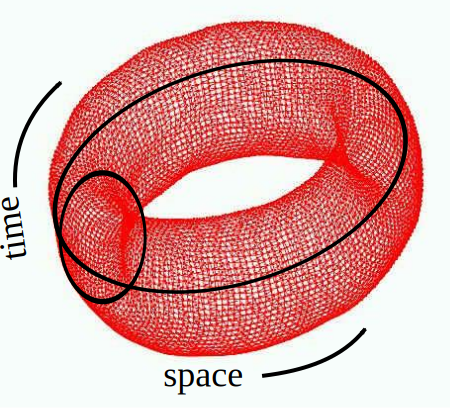
\includegraphics[width=.50\textwidth]{spaceTime1}
\\
\small{\texttt{(c)}}
\end{minipage}
    \end{center}
\caption{\label{fig:spaceTime1}
(a) A fixed $\speriod{}$ periodic spatial domain, all $\zeit$.
(b) A fixed $\period{}$ periodic temporal domain, all $\conf$.
(c) A fixed $\speriod{}\period{}$, doubly periodic spatiotemporally \twot.
}
\end{figure}
%%%%%%%%%%%%%%%%%%%%%%%%%%%%%%%%%%%%%%%%%%%%%%%%%%%%%%

    \PCpost{ 2016-10-11}{
{\bf Boris}
 has explained the strategy of {Ban} \etal\rf{BHLL13}, approach that he
himself has used: one constructs $\zeta$ functions for finite periodic domain
in one direction,
\ie, infinite strip $\mathbb{Z}_{\infty\times\speriod{}}$ or
$\mathbb{Z}_{\period{}\times\infty}$.
with a transfer operator generating the other, infinite
direction, as in \reffig{fig:spaceTime1}\,(b).
Those zeta functions are multiplied.
The infinite products, a different formula for each direction, describe the
same set of admissible patterns, resulting in some unexpected identities.

I find this very unnatural - intelligent zeta should account for all
commuting directions democratically.
    }

    \PCpost{2020-03-05}{
Douglas Lind's \HREF{http://faculty.washington.edu/lind/} {website}.

Lind\rf{Lind96}: Let $\map:X\to{X}$ be a homeomorphism of a compact space
and $N_n(\map)$ denote the number of points in $X$ fixed by $\map$. We
assume that $N_n(\map)$ is finite for all $n\geq1$.
$[\cdots]$
The zeta function has the product formula
\beq
\zetatop(z)=\prod_p\left(1-z^\cl{p}\right)
\ee{Lind96(1.2)}
where the product is over all finite orbits $p$ of $\map$ and $\cl{p}$
denotes the number of points in $p$.

To
compute $e_d(n)$ we use the Hermite normal form of an integer matrix
(see \refref{MacDuffee33}, Thm. 22.l).·

[10] Mac Duffee\rf{MacDuffee33} \emph{The Theory of Matrices}, (Chelsea, New York, 1956)
\CBlibrary{\rf{MacDuffee33}};
Y. Katznelson, Ergodic automorphisms of $T^n$ are Bernoulli, Israel J. Math. 10 (1971),
186-195.

The following question was suggested to us by David Ruelle:\\
\textbf{Problem 7.5}. Compute explicitly the thermodynamic zeta function
for the 2-dimensional Ising model, where $\alpha$ is the $\integers^2$
shift action on the space of configurations.
    }

    \PCpost{2021-07-28}{
Here is a cute ``interesting zeta function'' over $\integers$ with the
product formula, apparently known to Gauss:
\beq
\prod_n\frac{1}{1-z^n}=\sum_\ell p_\ell z^\ell
\ee{Lind96(1.3a)}
where  $p_\ell$ of is the number of partitions of   $\ell$.
    }

    \PCpost{2018-10-09}{
Lind and Schmidt\rf{LinSch02}
{\em Symbolic and algebraic dynamical systems},
\CBlibrary{LinSch02}
studies zeta functions for $\integers^d$ actions.
}

    \PCpost{2018-09-02, 2018-10-09}{
Einsiedler, Lindenstrauss, Michel and Ven\-ka\-tesh\rf{ELMV11} {\em Distribution
of periodic torus orbits and {Duke's} theorem for cubic fields}: ``
We study periodic torus orbits on spaces of lattices.  Using the action
of the group of adelic points of the underlying tori, we define a natural
equivalence relation on these orbits, and show that the equivalence
classes become uniformly distributed.  This is a cubic analogue of Duke's
theorem about the distribution of closed geodesics on the modular
surface:  suitably interpreted, the ideal classes of a cubic totally real
field are equidistributed {[...]}
''

{\em Homogeneous toral sets} do not seem to be defined. They generalize
the groupings of compact orbits (I believe these compact orbits are what
we call -at this moment- prime tori).

They define two invariants for homogeneous toral sets, {\em volume}
(defined in their eq.~(13), measuring how ``large" it is) and {\em
discriminant} (measuring its arithmetic complexity). I have no intuition
about what this discriminant is in our applications.

The periodic orbits are grouped into equivalence classes, equivalent
orbits having the same volume and discriminant.
An equivalence class of compact orbits is a \emph{packet}. Compact orbits
in the same packet have the same stabilizer and the same discriminant.
}

\item[2020-12-18 Predrag]
Esposti and Isola\rf{EspIso95} {\em Distribution of closed orbits for
linear automorphisms of tori} (1995) develop zeta functions for $d$\dmn\
tori; then they specialized to $D$ dof symplectic matrices acting on
$2D$\dmn\ tori, of which Isola's $d=2$ is a special case. But I'm
confused. I do not think that has to do with lattice zeta functions we
seek...

\item[2020-11-22 RSM]
The November 20, 2020 Matthew Gudorf {\em Spatiotemporal tiling of the
Kuramoto-Sivashinsky system} thesis dissertation defense interests me.
At the conceptual level it was already in
Pesin \& Sinai\rf{PesSin88} 1988 {\em Space-time chaos in the system of
weakly interacting hyperbolic systems},
for CML, and in my
MacKay\rf{MacKay12} {\em Space-time phases} 2012 lecture notes,
but claiming it applies to \KS\ is
bold. I suppose it does not fit perfectly, but interesting if it fits
approximately.

Is there a paper I can read?

\item[2020-11-22 Predrag] to Han: please read
MacKay\rf{MacKay12} {\em Space-time phases: {S}tatistical properties of
dynamics on large networks}
\HREF{https://thalis.math.upatras.gr/~phdsch11/wp-content/uploads/2011/05/MacKay-Lectures-STPhases.pdf}
{(click here)},
Sect.~2.2 {\em Statistical Phases for Uniformly Hyperbolic Attractors of
Finite-Dimensional Deterministic Dynamical Systems}
and related, and please take notes here on anything
that is related to our project.


\item[2020-12-16 RSM]
Cf. section~7.2.3 {\em Uniformly hyperbolic dynamics on networks}
in our {2013 LMS lecture notes}\rf{MacKay12} ``Masters of Complexity
Science'' \CBlibrary{MacKay12}.

\item[2020-12-16 Predrag]
Han Liang and I have been studying your {\em Space-time phases:
{S}tatistical properties of dynamics on large networks}\rf{MacKay12}, and
I was supposed to report back to you.
I like the proof of hyperbolicity for the {\spt} CML. Other than
\refsect{sect:chronotopic}~{\em Chronotopic literature}, this is the closest
to our {\spt} work.

\item[2020-12-16 RSM]
Perhaps the analogue of the MM formula that is relevant is the formula on
line 4 of p. 436, of which I am proud but it was also found by Bricmont
and Kupiainen, and they published before I did.

\item[2020-12-23 Predrag]
Bricmont and Kupiainen, \emph{High temperature expansions and dynamical
systems} \arXiv{chao-dyn/9504015}: `` We develop a resummed
high-temperature expansion for lattice spin systems with long range
interactions, in models where the free energy is not, in general,
analytic. We establish uniqueness of the Gibbs state and exponential
decay of the correlation functions. Then, we apply this expansion to the
{\FPoper} of weakly coupled map lattices.''

They credit
D. L. Volevich, \emph{Kinetics of coupled map lattices},
Nonlinearity 4, 37-45 (1991);
\emph{The Sinai -Bowen-Ruelle measure for a multidimensional lattice of
interacting hyperbolic mappings},
Russ. Acad. Dokl. Math.47, 117-121 (1993);
 and
\emph{Construction of an analogue of Bowen-Ruelle-Sinai measure for a
multidimensional lattice of interacting hyperbolic mappings},
Russ. Acad. Math. Sbornik 79, 347-363 (1994).

\item[2020-12-16 Predrag]
Spatially homogenous lattice models also invariant under discrete
\emph{space translations} were studied by Bunimovich and
Sinai\rf{BunSin88} in the case when  $g(\ssp_{n\zeit})$  is a one\dmn\
expanding map.

Regarding you ``symbol tables'' (what we call symbol {\brick}s): the
previous examples of ($D$+1)\dmn\ {\spt} symbolic dynamics: Pesin and
Sinai\rf{PesSin88}, Bunimovich and Sinai\rf{BunSin88}, Pethel, Corron and
Bollt\rf{PetCorBol06,PetCorBol07}. In other literature, I noticed that
Houlrik\rf{Houlrik92} gives Bunimovich and Sinai\rf{BunSin88} the credit.

The key insight\rf{BunSin88,GutOsi15} --an insight that applies to
coupled-map lattices\rf{PolTor92b,PetCorBol06,PetCorBol07}, and field
theories modeled by them, not only the system considered here-- is that a
field
\(
\Xx=\{\ssp_{z}\} % = \{\ssp_{z},  z\in \integers^{d}  \}
\)
over a $d$\dmn\ spacetime lattice $z\in \integers^{d}$ has to be
described by a corresponding symbol {\brick}
\(
\Mm=\{\m_{z}\} % = \{\m_{z}, z\in \integers^{d}\}
\,,
\)
over the same $d$\dmn\ spacetime  lattice $z\in \integers^{d}$, rather
than a 1\dmn\ temporal symbol sequence \refeq{linCode}, as one does when
describing a finite coupled ``$N$-particle'' system in the Hamiltonian
formalism.


Other than the ``symbol tables'', Bunimovich and Sinai\rf{BunSin88}
(1988) and Pesin and Sinai\rf{PesSin88} are profoundly different, nothing
to do with the {\spt} cat. Bunimovich has heard me talk about it, Sinai
not.

As \catlatt\ equations are symmetric under interchange of the `space' and
the `time' directions, their temporal and spatial dynamics are strongly
coupled, corresponding to $\epsilon \approx O(1)$ in \refeq{KanekoCML},
in contrast to the traditional spatially weakly coupled CML\rf{BunSin88}.

The conventional CML models start out with chaotic on-site dynamics
weakly coupled to neighboring sites, with strong spacetime asymmetry. In
order to establish the desired statistical properties of CML, such as the
continuity of their {SRB} measures, \refrefs{BunSin88,PesSin88} and most
of the subsequent mathematical literature rely on the structural
stability of Anosov automorphisms under small perturbations.
Contrast this with the non-perturbative $2$\dmn\ \GO\rf{GutOsi15}
{\em \catlatt} \refeq{LinearConn}.

Unlike the systems studied in \refref{BunSin88}, \catlatt\ cannot be
conjugated to a product of non-interacting  cat maps; a way to see that
is to compare the numbers of \twots\ in the two cases -- they differ.

In all other coupled maps literature I am aware of, the starting point is
time evolution of a non-interacting particle at each site, with its
1\dmn\ temporal symbolic dynamics, with spatial coupling to $D$ spatial
neighbors subsequently tacked on. While the spacetime \emph{coordinate}
of site is ($D$+1)\dmn, its symbolic dynamics is 1\dmn.

Your paper I found most eye-opening was the Hill's formula of\rf{MacMei83}
{\em Linear stability of periodic orbits in {Lagrangian} systems}.

We do not derive the formula the way you did it (ours also works for
dissipative systems), but the paper made the light bulb turn on...

Is there something else?

The thing we've been struggling with the most, that has kept the paper from a
publication is unimodular invariance of the defining cell (Bravais cell)
of a lattice (tiling of spacetime) so I have not been able to write down
a rational {\spt} topological zeta function in terms of prime
(non-repeating) 2-tori ({\spt} periodic orbits). Should be doable (the
Green's function is elliptic K function), but I just do not get it:)

\item[2020-12-16 RSM]
Yes, neat to consider cat map as a second order recurrence on one
variable rather than a first order one on two variables (I hadn't
appreciated the advantage when Vivaldi was talking about it way back
then) and then it indeed looks like a discrete field theory and extends
naturally to space-time and you can code all solutions by lattices of
integers, one for each point in space-time.

In the general ``uniformly hyperbolic'' situation (in quotes because it
is the way to connect with dyn sys, but the point is to escape from
time-evolution view, as you do, and consider solutions as being zeroes of
some function from states on {\spt} lattice to the {\spt} lattice and
then u hyp just means the derivative of the function has bounded
inverse), expect to be able to code all solutions by some set of allowed
symbol tables, via {\spt} shadowing (which is just shadowing in the more
general context, again having nothing to do with time-evolution).  Not
sure to what extent I mentioned this in my lecture notes, but perhaps it
appears in the article I wrote for Chazottes \& Fernandez earlier.  I have
certainly waved {\spt} shadowing around as providing an answer, but never
really done it for any particular system.  Will think about it.

Will also think about your question of zeta fn for the Gutkin-Osipov CML.
It will be a straightforward answer once we have thought of it, but a
question of keeping everything straight in one's mind.  I'm not clear
where your obstacle is.  We can count all {\spt} periodic solutions and
so make a zeta fn; you want to reduce it to an expression in terms of
prime ones? or to one in terms of collections of disjoint elementary
cycles? (I put elementary in there because graph theorists use closed
walk for what you might call a cycle and cycle for what I'm calling an
elementary one)  ``Just'' need to work out the {\spt} analogue.  Maybe I
need to wake up fresh tomorrow morning to do it.  Or have a whisky now to
do it (except I don't have any in the house right now!).

\item[2020-12-17 RSM]
I found the \PV\rf{PerViv} paper (having first found their other
one\rf{PerViv87b} from 1987 on the periodic orbits).
As I remembered, they do not appear to derive finite-type conditions on
their coding.  I suspect it is not of finite type.  Thus I'd say it is
pretty useless, compared to the \AW\ partition.

I wasn't convinced by  \PV\rf{PerViv} as it is not obvious (to me) what
are the constraints on the sequence of integers $m_t$.  Do you know?  Say
we take
\(
   \phi_{t+1}-3\phi_t+\phi_{t-1}=0\;\mod 1,\; \phi \in [-1/2,1/2)
\)
then we can get $\{-2,-1,0,1,2\}$, but not all sequences of such integers
are possible because that would give entropy log 5 whereas it is supposed
to be $\log(3+\sqrt{5})/2$, or
$\log(s+\sqrt{(s-2)(s+2)})/2$ in general.
There should be a simple finite-type condition. Do you know it?

\item[2020-12-18 Predrag]
I agree. It's ridiculous, arbitrary frame on the unit torus, contra
natura, ignoring stable/unstable manifolds, painful to implement –
Dirichlet conditions destroy the time-translational invariance of the
lattice. That is why I included
\HREF{http://chaosbook.org/overheads/spatiotemporal/GHJSC16.pdf\#figure.2}
{figure 2} and
\HREF{http://chaosbook.org/overheads/spatiotemporal/GHJSC16.pdf\#table.2}
{table 2} – an impossible
number-theoretic problem created by ignoring the well-known generating
partition construction. There Vivaldi and Percival got it wrong.

Aside: Nobody listens to me, and in particular Russians, so I had to
watch and assist Gutkin and 3 grad students push this pointless torture
of a paper. The problem is that quantum chaos crowd profoundly lacks
understanding of periodic orbit theory – I wrote a whole book to explain
that periodic orbit calculations are general nonlinear coordinate
transformation invariant, that one does not need nowhere differentiable
probability measures, to no avail. Russians make it worse by idolizing
Sinai and believing that one has to construct explicit,
coordinate-dependent generating partitions – that never works except in 3
or so examples which are the only ones they are always taught.

\item[2020-12-17 RSM]
Do you have a way around it?

\item[2020-12-18 Predrag]
Yes, we construct the \AW\ generating partition for \PV\ 2-configuration
map in ChaosBook.org (not polished yet, but for you I've promoted it from
internal to publicly readable text):
\toChaosBook{exmple.14.12}{Example 14.12} {\em Adler-Weiss partition of
the cat map state space.} Our construction is sufficiently clever that my
very smart collaborator Gutkin still does not get it:)

While Percival and Vivaldi were well aware of \AW\ partitions, they felt
that their ``coding is less efficient in requiring more symbols, but it
has the advantage of linearity.'' Our construction demonstrates that one
can have both:  an \AW\ generating cat map partition, and a linear code.
The only difference from the \PV\ formulation\rf{PerViv} is that one
trades the single unit-square cover of the torus of
\refeq{eq:StateSpCatMap} for the dynamically intrinsic, two-rectangles
cover, but the effect is magic - now every
infinite walk on the {\markGraph}
corresponds to a unique {\admissible} orbit $\{\ssp_{\zeit}\}$, and the
{\markGraph} generates all {\admissible} itineraries $\{\Ssym{\zeit}\}$.

But the Hamiltonian formulation is stupid. The great advantage of the
Lagrangian, temporal lattice formulation is that the fundamental fact
yields the number of periodic solutions and the zeta function without any
explicit time-evolution generating partition. I believe that explicit
time-evolution generating partitions are impossible to generalize to
spatial lattices evolving in time.

\item[2020-12-17 RSM]
You cited Isola\rf{Isola90} for the {$\zeta$}-function  for the cat map
but I thought people like Manning had calculated it earlier.  I looked up
his 1971 paper on rationality of zeta for Axiom A and see he cites
Smale's 1967 review for toral automorphisms.

\item[2020-12-18 Predrag]
I doubt it. In his 1971
{\em {Axiom A} diffeomorphisms have rational zeta function}\rf{manning}
he explains rationality of topological (orbit counting)
of Smale's school zeta functions in terms of `Manning multiples',
what I understand as
inclusion-exclusion principle (when sets share boundaries, boundary has
to be –recursively- subtracted not to be overcounted).

It is easy enough
to construct, but I have not seen cat map zeta function earlier than the
one written down by Isola. Will change the citation if we find an earlier
one.

\item[2020-12-18 RSM]
OK, you map the \AW\ partition into $(x,x')$ coordinates and then reduce by
translation into that fundamental domain instead of the standard one.
Got it.  I thought you had some magic for the standard fundamental
domain.
I agree the tedious thing about counting periodic orbits of toral
automorphisms is the ambiguity of coding for orbits on the partition
boundaries.  A cute thing is that if you consider the map on a sphere
(with 4 conical points) induced by quotienting by reflection through 0,0
then you get exactly $\tr A^n$ fixed points of $A^n$, see
Llibre and MacKay\rf{LliMac92} {\em {Pseudo-Anosov} homeomorphisms on a
sphere with four punctures have all periods} (1992).

\item[2020-12-18 Predrag]
A very cute paper, but it will not help me here, will it?

\item[2020-12-18 RSM]
OK, I might look up Pollicott on zeta fns for toral autos because I think
he has some lecture notes in which he gives history.

On your big question, can I phrase it as how many orbits under
$\SLn{2}{\integers}$ are there for its action on integer parallelograms of
given area (based at 0)?  Equivalently, how many sublattices of given
area are there in $\integers^2$?

\item[2020-12-18 Predrag]
It's the first step, a warm-up exercise - we all can do it.
But then you have to count the number of \twots\ that live on each
parallelogram. The paper explains that we know how to do it,
but if we had the zeta functions, it would generate all these numbers.

It could be that the sensible zeta function is
a double series in $(z_1^\speriod{},z_2^\period{})$, in which case we
want to count integer parallelograms of periods
$(\speriod{},\period{})$, not lump them into areas
$A=\speriod{}\period{}$, and have a zeta function which is a series in
single $z^A$.

\item[2020-12-18 RSM]
It is the sort of thing Marklof probably knows.  But we can think about
it too.  For area 1 I get 1 because I can map any unit parallelogram to
the unit square by the inverse of the matrix representing its sides,
which is in \SLn{2}{\integers}.  For area 2, I think I get two, by
observing that to have area 2, the matrix has one row or column divisible
by 2 and then dividing that out and using its inverse to map to one of
the two standard rectangles.  For area 3 I didn't get an answer yet.  But
I wonder if it is something trivial like the area.  This would fit with
your fundamental fact.

\item[2020-12-18 RSM]
I see I was wrong in getting only two orbits of parallelograms for area
2.  There's also the diamond.  I must have missed something with the rows
and columns calculation (which admittedly I did while in bed)!  Ah yes, I
remember I did see one more solution and then forgot it by the time I go
up. {Here it is done properly}:

\begin{quote}
\HREF{https://math.stackexchange.com/questions/2368026/number-of-sublattices-of-bbb-z2}
{Number of sublattices of $\integers^2$}. ``I would like to count the
number of sublattices $\lattice$  of $\integers^2$ of index
$n=|\det\lattice|$.''
\end{quote}

\item[2020-12-19 Predrag] This example lists $\det\lattice=2$ parallelograms
as (columns
are their basis vectors)
\beq
\left[
\begin{array}{cc}
 2 & 0 \\
 0 & 1 \\
\end{array}
\right]
,\,
\left[
\begin{array}{cc}
 0 & 1 \\
 2 & 0 \\
\end{array}
\right]
,\,
\left[
\begin{array}{cc}
 1 & -1 \\
 1 &  1 \\
\end{array}
\right]
\,.
\ee{RSM-1}
The third one is not in the Hermite normal form, but presumably a unimodular
transformation (have not checked it) brings it to the upper diagonal
form $\BravCell{2}{1}{1}$ \twot\ that we use.

This example counts
parallelograms under distinct translations (must make sure that each unimodular
orbit is counted only once).
Guido, Isola and Lapidus\rf{GuIsLa08} (or
\toChaosBook{chapter.25}{chapter 25} \emph{Discrete symmetry
factorization}) count parallelograms distinct under reflections.

I think counting $\det\lattice=A$ parallelograms is easy.
What we need is a generating function that counts numbers of \twots, and
the related zeta that counts the numbers of \emph{prime} \twots.

\item[2020-12-18 Predrag]
If it is any help, for small areas answers are listed in
\HREF{http://chaosbook.org/overheads/spatiotemporal/CL18.pdf\#table.2}
{table 2}.

\item[2020-12-18 RSM]
The question is how to make a zeta fn from these counts.  Take simplest
case of Bernoulli on ${s}$ symbols.  For each area n, we have $T_n = \sum d$
over divisors of n, sublattices.  Each can be populated by ${s}^n$ patterms
(not worrying about patterns with a smaller lattice), so there are ${s}^n
T_n$ patterns with an area n.  I suppose it is natural to divide by $n$
because we could move the origin to any of the n points.  So propose
\(
\zeta(z)=\exp \sum_n {s}^n z^n T_n/n
\)
for this example.  Need to look up some
number theory to simplify this but I think it is some standard formula.

\item[2020-12-18 RSM]
Ah, I see from (86) of your draft paper that I have made a mistake.  Yes,
have identified my error now. Here is
\HREF{https://math.stackexchange.com/questions/273275/generating-function-for-the-divisor-function}
{a useful page}.
So, OK, number of Bravais lattices has zeta fn (with respect to area) =
$\prod_L (1-z^L)$.  But you already knew this.  Your question at the bottom
of p. 21 is to count prime lattices or perhaps the more subtle one of
counting prime periodic patterns taking the finite-type conditions of
{\spt} cat into account.

\item[2020-12-19 RSM]
% Not sure if it is what you want but
If define $\zeta(z)=\exp \sum_n z^n/n N_n$ where $N_n$ is the number of
{\lattstate}s that have a period parallelogram of area n, and we let
prime patterns be ones that are not repetitions of ones with a smaller
area, and regarded as equivalent if differ by a translation, then I get
\(
\zeta(z) = \prod_\gamma F(z^{|\gamma|})
\)
over {\orbit}s $\gamma$, where $F(x) = \prod_m (1-x^m)^{-1/m}$. Not
sure if F can be simplified.

\item[2020-12-16 Predrag]
We have not been able to make that one work. Square lattice is separable,
so one hopes for something like that. The problem is that in the addition
to double periodicity, there is a third integer – parallelogram come with
different tilts (screw bc's). Some details are towards the end of the
current draft\rf{CL18},
	Predrag Cvitanovi\'c and Han Liang \emph{Spatiotemporal cat: A
chaotic field theory} rough draft, (November 2020) on
\HREF{http://ChaosBook.org/overheads/spatiotemporal/index.html}
{\spt\ homemade}.

\item[2020-12-20 RSM]
I have some thoughts about the 2D $\zeta$ function, in particular the
question of how to generalise $\det (I-zW)$ from finite type conditions
(or more generally weights $W$) for nearest nbr chains to finite type
conditions (or more generally weights from cliques) for 2D lattices.  I
think it proceeds in same way as I did for Gibbs measures for CML.

\item[2020-09-24, 2020-12-16 Predrag]
My thoughts in that directions (that is in my \catlatt\ talk,
and in this blog, see
\refeq{FGHLW74:charFunct1d},
\refeq{AABHM99-56a},
\refeq{AABHM99-56d},
\refeq{PCcatLattZeta1})
are that for the 2\dmn\ {\catlatt}\rf{GHJSC16,CL18}
\beq
       \ssp_{n,\zeit+1} + \ssp_{n,\zeit-1}
- 2{s} \, \ssp_{n\zeit}
     + \ssp_{n+1,\zeit} + \ssp_{n-1, \zeit}
     = -\Ssym{n\zeit}
\,,\qquad \Ssym{n\zeit}\in\A
\,,
\ee{CatMap2dRSM}
with alphabet
\beq
 \A  =
 \{-{3},-{2},-{1},
   0,\cdots,
   {\mu}^2+1,{\mu}^2+2,{\mu}^2+3\}
\,,
\ee{catLatt2dRSM}
and the Yukawa mass squared of the scalar field $\ssp$
\beq
   {\mu}^2 = 2({s}-2)
\,.
\ee{catlattMassRSM}
The $\zeta$ function has to satisfy all {\spt} symmetries of the square
lattice \refeq{eq:D4}
\beq
C_{4v} = \Dn{4} = \{
E, C_{4z}^+, C_{4z}^-, C_{2z},
\sigma_{y}, \sigma_{x},
\sigma_{a},\sigma_{b}
\}
\,.
\ee{eq:C4v}
See \toChaosBook{section.Y.1} {sect.~A25.1}.

In the international crystallographic notation, this square lattice space
point group is referred to as $p4mm$\rf{Dresselhaus07}.

\item[2020-12-16 Predrag]
The simplest rational $\zeta$ function that satisfies these symmetries is
of form
\beq
  \zetatop(z_1,z_2)
=
  {d({s})}/{d(2)}
=
  1 - {{\mu}^2}/{d(2)}
\,,
\ee{zetaCatLattRSM}
where
\beq
   d({s}) = {z_1 + z_2 - 2{s} + z_1^{-1} + z_2^{-1}}
\ee{LaplCatLatt}
$d({s})$ is the Z-transform (discrete Laplace transform) of
\refeq{CatMap2dRSM}. Fischer \etal\rf{FGHLW74} call this the
\emph{characteristic function}, a somewhat over-abused nothing-saying
appellation.

Anything more complicated would be a disappointment :)

\item[2020-12-20 Predrag]
Its massless ${\mu}^2=0$, Poisson equation value $d(2)$  is the
Z-transform of the $d=2$ lattice Laplacian. $d({s})$ can be written in a
\Dn{4}-symmetric form
\bea
   d({s}) &=& { (1 - \ExpaEig z_1)(1/z_1 - 1/\ExpaEig)
               +(1 - \ExpaEig z_2)(1/z_2 - 1/\ExpaEig)}
\continue
   d(2) &=& {(1 - z_1)(1/z_1 - 1)+(1 - z_2)(1/z_2 - 1)}
\,.
\label{LaplPoiss}
\eea
Here $(\ExpaEig,1/\ExpaEig)$ are the roots of
the $d=1$ {characteristic equation}
\beq
\ExpaEig^{2} - {s}\ExpaEig + 1 = 0
\,,
\ee{diffEqs:StabMtlprRSM}
which, for $|s|>2$, has two real roots
% stability multipliers
$\{\ExpaEig\,,\;\ExpaEig^{-1}\}$,
\beq
\ExpaEig
=\frac{1}{2}(s+\sqrt{(s-2)(s+2)})
\,,
\ee{PCStabMtlprRSM}
\beq
\ExpaEig
=\frac{1}{2}(\mu^2+2+\mu^2\sqrt{1+\left(\frac{2}{\mu}\right)^2})
\,,
\ee{PCStabMtMu}
\beq
s
  = \ExpaEig+\ExpaEig^{-1}
  = e^\Lyap+e^{-\Lyap}
  = 2\cosh\Lyap
\,,\quad \Lyap>0
\,.
\ee{catMapEig1}


Derivatives, integrations with respect to the parameter $(z_1,z_2)$,
should relate this to the numbers of {\lattstate}s generating
function, but Han, my graduate student, tells me that does not work.
Perhaps, in the spirit of Schwinger and Feynman `tricks'
derivatives, integrations with respect to the stretching parameter ${s}$
or squared mass $\mu^2$ do the job.

Decomposition \refeq{LaplPoiss} is dodgy - in higher dimesnions there
are other eigenvalues than \refeq{PCStabMtlprRSM}.

\item[2020-12-17 RSM]
I found [...] \PV\rf{PerViv} [... see above ...]
There should be a simple finite-type condition. Do you know it?

\item[2020-12-20 Predrag]                               \toCB
As for the {cat map}, we split the ${\mu}^2+7$ letter alphabet $\A=\Ai\cup\Ae$
into the interior \Ai\ and exterior \Ae\ alphabets\rf{GHJSC16}
\beq
  \Ai=\{0,\dots,{\mu}^2\},   \quad
  \Ae=
\{-{3},-{2},-{1}\}\cup
\{{\mu}^2+1,{\mu}^2+2,{\mu}^2+3\}
\,.
\ee{2dCatLattAlphRSM}
For example, for ${\mu}^2=1$ (ie, $s=\edit{5/2}$) the interior,
respectively exterior alphabets are
\beq
  \Ai=\{0,1\},   \quad
  \Ae=\{-{3},-{2},-{1}\}\cup \{2,3,4\}
\,.
\ee{2dCatLattAlph5RSM}
If all $\Ssym{z}\in \Mm$ belong to \Ai, $\Mm$ is
{\admissible}, i.e., $\Ai^{\integers^2}$ is a full shift\rf{GHJSC16}.
    \PCedit{
All grammar rules involve exterior alphabet \Ae. I do not know whether
there is a finite grammar, or the grammar is the infinite one investigated
by Gutkin \etal\rf{GHJSC16}. My claim is that it does not matter, as
we know how to count all $\LTS{}{}{}$, and for each we can read off
all admissible {\Mm} by listing all integer points within the $\jMorb_\Mm$
{\fundPip}.
    }

Curiously, even the Poisson ${\mu}=0$  case looks chaotic, numerically
(though how would our graduate students notice logarithmic corrections
due to the 0-mode?), see
\HREF{http://chaosbook.org/overheads/spatiotemporal/GHJSC16.pdf\#figure.5}
{figure 5\,(c)} of Gutkin \etal\rf{GHJSC16}.
That presumably arises from the intersection set (the boundary)
of the \refeq{dynD_1} fundamental domain and its reflection.








\end{description}

\renewcommand{\ssp}{x}
\renewcommand{\Ssym}[1]{{\ensuremath{s_{#1}}}}    % Boris
%%%%%%%%%%%%%%%%%%%%%%%%%%%%%%%%%%%%%%%%%%%%%%%%
\printbibliography[heading=subbibintoc,title={References}]
